\chapter{Estimating geographic location}
\label{chapter_est_geoloc}
In order to evaluate the performance of longitude and latitude estimation functions, it may prove useful to be able to translate the error values from degrees to kilometers. The following two Equations \ref{equation_latitude_delta_km} and \ref{equation_longitude_delta_km} can be used to approximate the deltas of longitude and latitude estimation functions in kilometers. Note that these functions are only approximations as they rely on the assumption that the Earth is a perfect sphere and not an irregular ellipsoid.


\hfill \break
%%%%%%%%%%%%%%%%%%%%%%%%%%%%%%%%%%%%%%%%%%%%%%%%%%%%%%%%%%%%%%%%%%%%% START
\noindent\textbf{Latitudinal distance to kilometers}(Distance on North-South axis)
%
\begin{equation}
\begin{split}
\label{equation_latitude_delta_km}
Distance_{latitudinal}(lat\_d)=(40 000km/360^\circ)* lat\_d
\end{split}
\end{equation}

\noindent Where 

$lat\_d$ is the distance between two points in degrees latitude and 40000km is an approximation for Earths circumference.

\vspace{5mm} %5mm vertical space
%%%%%%%%%%%%%%%%%%%%%%%%%%%%%%%%%%%%%%%%%%%%%%%%%%%%%%%%%%%%%%%%%%%%% END

%%%%%%%%%%%%%%%%%%%%%%%%%%%%%%%%%%%%%%%%%%%%%%%%%%%%%%%%%%%%%%%%%%%%% START
\noindent\textbf{Longitudinal distance to kilometers at given latitude}(Distance on East-West axis)
%
\begin{equation}
\begin{split}
\label{equation_longitude_delta_km}
Distance_{longitudinal}(lon\_d, lat)=(40 000km/360^\circ)* cos(lat)*lon\_d
\end{split}
\end{equation}

\noindent Where 

$lon\_d$ is the distance in degrees longitude and $lat$ is the latitude for which the distance is calculated.



\vspace{5mm} %5mm vertical space

\noindent As long as the deviations are small enough and highly accurate error values are not needed, the total error in absolute terms can be estimated by using the latitudinal and longitudinal distances as the x and y coordinates on a cartesian plane and computing the euclidean distance between the origin and resulting point.

%%%%%%%%%%%%%%%%%%%%%%%%%%%%%%%%%%%%%%%%%%%%%%%%%%%%%%%%%%%%%%%%%%%%% END

\newpage
\section{Estimating geographic longitude}
\noindent As mentioned in Sections \ref{section_different_latitudes} and \ref{section_different_longitudes}, the geographic location of a PV system has a strong correlation to the timing of the first and last non-zero measurements of each day whereas the influence of tilt and facing parameters seems to be nonexistent. The relationship would seem to be so clear that without further analysis it would be tempting to use fairly simplistic mathematical models for these estimations. The following longitude estimation Function \ref{equation_naive_longitude} can be derived with two assumptions. These assumptions are that solar noon occurs at 12:00 or 720 minutes at longitude 0 each day and at 6:00 or 360 minutes at 90 degrees. Rest of the values can then be linearly interpolated. Note that here solar noon refers to the midpoint between the first and last non-zero minute which is different from astronomical solar noon which occurs nearly at the same time.

As only the first and last non-zero minute times are relevant for longitude and latitude estimation, PVlib POA model is used for both longitude and latitude estimation.

\hfill \break


%The simpler of these relationships is the relationship between the longitude and first and last non-zero minute times. Based on the figure \ref{fig-poa_var_lon2}, this relationship seems to be very close to linear. This makes the use of a simple linear equation rather compelling. 



%%%%%%%%%%%%%%%%%%%%%%%%%%%%%%%%%%%%%%%%%%%%%%%%%%%%%%%%%%%%%%%%%%%%% START

\noindent\textbf{Naive solar noon to longitude equation}
%
\begin{equation}
\begin{split}
\label{equation_naive_longitude}
Longitude(sn)=180^\circ-\frac{360^\circ}{1440}*sn
\end{split}
\end{equation}
Where $sn$ is the approximated solar noon minute calculated by taking the average of first and last non-zero power generation minute of a day. % $0.25$ or $360/1440$ corresponds to the longitude degrees per minute and $180$ is used as offset value. This naive equation assumes that solar noon occurs at 12:00 or 720 minutes each day at $0^\circ$ longitude. Note that here solar noon refers to the midpoint between the first and last non-zero minute which is different from astronomical solar noon which occurs nearly at the same time.

\hfill \break
%%%%%%%%%%%%%%%%%%%%%%%%%%%%%%%%%%%%%%%%%%%%%%%%%%%%%%%%%%%%%%%%%%%%% END


\noindent The simplicity of Equation \ref{equation_naive_longitude} makes the equation appealing, but the assumption of solar noon occuring at 720 minutes should still be verified. In Figure \ref{fig_solarnoons} solar noons can be seen to occur at around 720 minutes at longitude 0 but they can also be observed occuring 15 minutes earlier or later than that. This 15 minute delta would translate into an error range of $(\pm 15/1440)*360^\circ = \pm 3.75^\circ$ degrees or approximately $\pm 200 km$ at the latitudes of Helsinki according to the Equation \ref{equation_latitude_delta_km}.


Knowing that the PV installation is within a 400 kilometer wide slice should be in most cases be accurate enough for determining the country in which the PV installation is located in, but for most other purposes this level of accuracy is unlikely to be valuable. Fortunately the naive model can be improved upon by taking the solar noon timing variation into account. \hfill \break

\begin{figure}[ht!]
\centering
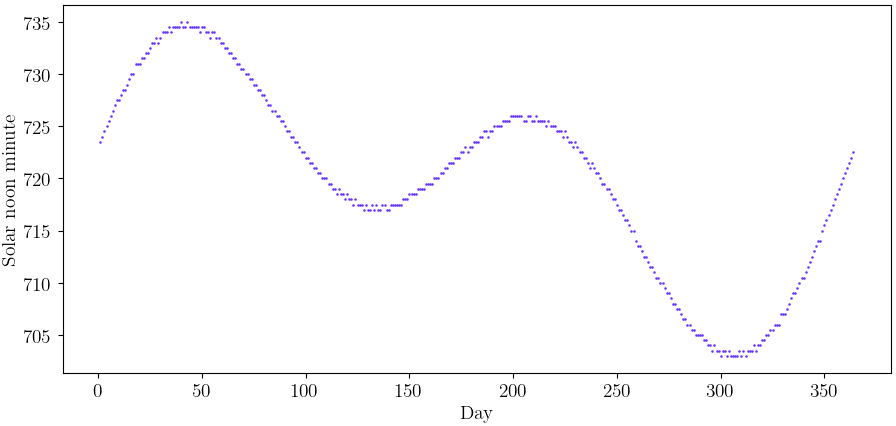
\includegraphics[width=1\linewidth]{pics/solarnoons2}
\figcaption{Approximations of solar noon minutes based on PVlib POA function at longitude $0^\circ$ for year 2023. This pattern is caused by the difference in solar time and UTC time \cite{eot}.}
\label{fig_solarnoons}
\end{figure}



\newpage
%%%%%%%%%%%%%%%%%%%%%%%%%%%%%%%%%%%%%%%%%%%%%%%%%%%%%%%%%%%%%%%%%%%%% START
\noindent\textbf{Improved longitude estimation function }
%
\begin{equation}
\begin{split}
\label{equation_longitude_estimation_2}
Longitude(sn)= \frac{360}{1440}(sn_{poa}-sn)
\end{split}
\end{equation}

\noindent Where $sn$ is the solar noon estimate based on measurement data and $sn_{poa}$ is the simulated solar noon at $0^\circ$ longitude. The new function parameter $sn_{poa}$ compensates for the variation seen in Figure \ref{fig_solarnoons}.


%%%%%%%%%%%%%%%%%%%%%%%%%%%%%%%%%%%%%%%%%%%%%%%%%%%%%%%%%%%%%%%%%%%%% END

\vspace{5mm}


\noindent
%The improved function \ref{equation_longitude_estimation_2} should be much more accurate than the earlier longitude function. as the errors in estimates should primarily be the result of bias in the measurements data.


%In figure \ref{fig_solarnoons_poa_vs_measurement} the solar noon estimates calculated by taking the average of first and last non-zero minute of the day can be seen to preceed the solar noons by roughly 8 minutes. This systematic bias could be explained by the east facing orientation of the panels and correcting for the bias could could be fairly difficult. 

\vspace{0.5cm}
%The theoretical accuracy at this stage could be as high as $\frac{360^\circ}{1440} = 0.25^\circ$ but 
\noindent The improved algorithm should no longer have a systematic error of up to 15 minutes after the difference between solar time and UTC time variation has been taken into account. In addition to correcting for the irregular solar noon timing, the algorithm can be improved even further by using it on larger sections of data and averaging the results, or alternatively, the algorithm could be applied only on selected cloud-free days where the expected errors are likely to be smaller.

If the unfiltered multi-day approach is used, choosing the right day range is crucial. If the range is too narrow, a single outlier value can distort the results significantly, however if the whole year is used, certain periods of the year may contain more noise than others and thus their use could decrease the accuracy of the results. The two scatterplots in Figure \ref{fig_first_last_kuopio_helsinki} show that the data quality from the very first and last days of the year seem to be significantly worse than the data from the longest days of the year. Based on these visualizations, days inside the range 100th to 280th would seem best suited for first and last minute sensitive analysis algorithms for both Helsinki and Kuopio installations.



%noise present in non-zero minutes is higher in the Kuopio installation data. 

%noise present in power generation measurements may result in significant errors in estimates based on individual days. These errors can be mitigated by using the algorithm on larger sections of data and averaging the results, or alternatively the algorithm could be applied only on selected cloud free days where the expected errors are likely to be smaller. If the unfiltered multi-day approach is used, choosing the right day range is crucial. If the range is too narrow, a single outlier value can distort the results significantly, however if the whole year is used, certain periods of the year may contain more noise than others and thus their use could decrease the accuracy of the results. The two scatterplots in figure \ref{fig_first_last_kuopio_helsinki} show that the data quality from the very first and last days of the year seem to be significantly worse than the data from the longest days of the year. The same graph would also seem to suggest that overall data quality decreases the further north the installation is. Based on these visualizations, days outside the range of 100th to 280th would seem unsuitable for first and last minute based analysis between latitudes $60^\circ N$ and $63^\circ N$.


\begin{figure}[ht!]
\centering
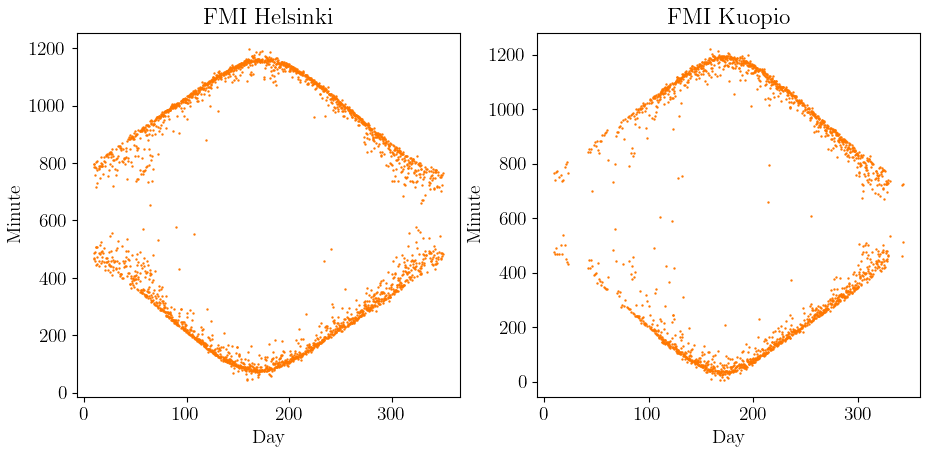
\includegraphics[width=0.9\linewidth]{pics/first_last_helsinki_kuopio2}
\figcaption{First and last non-zero power minutes of each day during years 2017 to 2021 from FMI Helsinki and Kuopio datsets.}
\label{fig_first_last_kuopio_helsinki}
\end{figure}

\clearpage

\subsection{Longitude estimation results}
The improved algorihm was tested on the day range of 125th to 250th of each year from both FMI datasets and the results can be seen on the Table \ref{table_geolocator_results}. For the Helsinki installations these estimates are all off by less than $0.3^\circ$ while as the Kuopio installation deltas are a bit higher with max of just over $1^\circ$. More impressively, the mean delta of multiple years for the Helsinki dataset is just $0.07^\circ$ and $0.46^\circ$ for Kuopio. In kilometers, the mean deltas can be approximated to 4 and 28 kilometers respectively. The lower accuracy of the Kuopio estimations could be due to multitude of factors ranging from differences in local climate or lower elevation of the installation among others. 




\begin{table}[ht!]%[!h]
\centering
\begin{tabular}{r|c|c|c|c} \hline\hline

 Year & Longitude Helsinki & $\Delta^\circ$  & Longitude Kuopio & $\Delta^\circ$ \\ \hline
 2021 & $25.115^\circ$  & $0.154^\circ $  & $26.625^\circ$ & $-1.009^\circ $ \\
 2020 & $25.029^\circ$ & $0.068^\circ $& $27.691^\circ$  & $0.057^\circ $ \\
 2019 & $24.944^\circ$ & $-0.017^\circ $& $27.411^\circ$ & $-0.223^\circ $  \\
 2018 & $25.243^\circ$ & $0.282^\circ $& $26.862^\circ$ & $-0.772^\circ $ \\
 2017 & $24.836^\circ$  & $-0.125^\circ $& $27.297^\circ$ & $-0.337^\circ $ \\
 mean & $25.031^\circ$  & $0.07^\circ $& $27.177^\circ$ & $-0.457^\circ $ \\
\hline\hline
\end{tabular}
\tabcaption{Means of multi-day longitude estimations from 125th to 250th day of each year.}
\label{table_geolocator_results}
\end{table}

\newpage
\subsection{Possible issues and further development ideas}
While experimenting with the solar minute estimation functions, a curious trait was found. In Figure \ref{fig_solarnoontimes}, the average of the first and last minute is approximately the same for each day at different latitudes as long as the latitude is below 50 degrees. As the latitude is increased, the solar noon estimates begin to deviate significantly, becoming strongly skewed after 70 degrees. 

At first this behavior seems strange as astronomical solar noon should occur happen at the same time when longitude and the day are the same regardless of latitude. However as the solar noon estimates are calculated based on the first and last non-zero irradiance minute of the day, it would make sense that the estimations could be off by significant amount during equinoxes due to rapid changes in day lengths. Measuring out how significantly this affects longitude estimations is challenging. In theory, if the same bias occurs in both the measurements and the model, no corrections would be needed. The effect should be also lessened by using longer day ranges for predicting longitudes or by making sure that the intervals include an equal amount of days from both halves of the year. 

Improvements in the algorithm accuracy could also be achieved via by increasing the sampling interval of the irradiance simulations. PVlib POA simulations include a parameter for sampling frequency which is currently set to 1-per-minute in order to match the measuring frequency of FMI datasets. This could be increased to 1-per-second and the added resolution could help in determining more accurate estimates for solar noon times, resulting in possible gains in algorithm accuracy.

PVlib POA model was used instead of the more complex reflection and temperature aware model. This could be done as the geolocation is connected to first and last non-zero minute times which should be the same for both models. However even the POA model might be overly complicated as only two time values are needed.




\begin{figure}[]
\centering
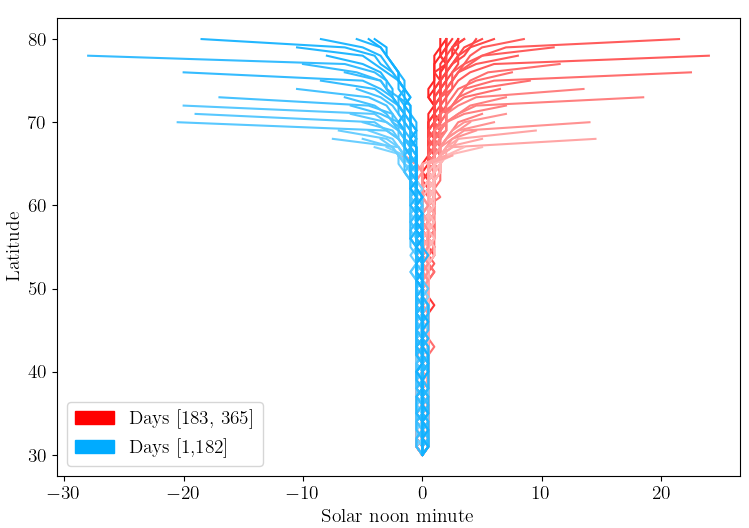
\includegraphics[width=1\linewidth]{pics/solarnoontimes2}
\figcaption{Relationship between latitude parameter and estimated solar noon time. Each line represents a different day of the year and x-axis values are normalized so that each line begins at 0 deviation. Lines with darker colors mark days which are further away from spring and fall equinoxes.}
\label{fig_solarnoontimes}
\end{figure}







%\textbf{Longitude estimation notes}

\newpage 
\section{Estimating geographic latitude}
Similarly to the longitude, the latitude of an installation is strongly connected to the timing of the first and last non-zero minutes of the day. This means that PVlib POA simulations can be used instead of the more complex PV model.

In Figure \ref{fig_poa_var_lat}, the simulated first and last minutes can be seen to change day by day at varying rates based on the latitude. In mathematical terms it could be said that the slope of the day-to-first-minute function is determined by the latitude of the installation. And for the days around equinoxes, and at higher latitudes of $50^\circ$ to $70^\circ$, this relationship would seem to be bijective as per earlier Figure \ref{fig_poa_var_lat}. The followinth algorithm is based on the former observations.


\hfill


\subsection{Latitude algorithm}
%\noindent\textbf{Latitude algorithm}
\begin{enumerate}
  \item Simulate first non-zero minutes over a specific day range at a given latitude.
  
  \item Fit a linear equation to the simulated day to first minute pairs from step 1.
  
  \item Repeat steps 1 and 2 for multiple latitudes and graph the relationship between days and first minutes.
  
  \item Fit a line to the graph from step 3 and save the line slope.
  
  \item Create a slope to latitude graph.
  
  \item Fit an n-degree polynomial equation to the graph from step 5.
  
  \item Calculate the slope of first minutes for real measurement data over the same range as was done in step 1 and use the slope as input for polynomial from step 6. The value of the polynomial is the estimated latitude.
  
\end{enumerate}

\noindent
\textbf{Notes:}
%A visualization of the algorithm can be seen in the following figure \ref{fig_slope_to_latitude}. 
Due to seasonal differences in data quality, polar winters and the midnight sun, the range of days chosen for the algorithm is important. If the range is short, individual outliers in measurements can result in large errors. Whereas if the range is too long, it will be harder to choose the range while avoiding low data quality sections. In the algorithm visualization Figure \ref{fig_slope_to_latitude}, the range of 250th to 300th seems to result in acceptable slope to latitude curve smoothness.
\newpage

%\subsection{Latitude algorithm visualization}
\begin{figure}[ht!]
\centering
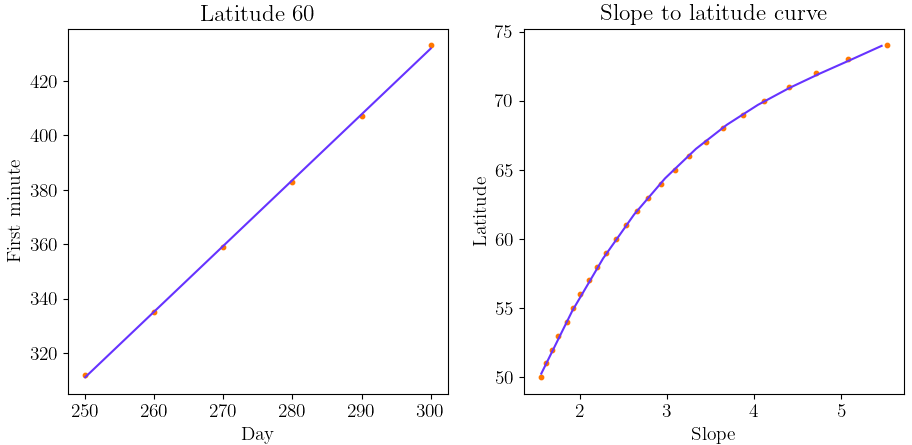
\includegraphics[width=1\linewidth]{pics/slope_to_latitude3}
\figcaption{Left shows the linear relationship between day and simulated first minutes. Right shows the relationship between the slope angle and latitude.}



%the latitude algorithm steps 1 and 2 for day range 250 to 300 at latitude 60 and the linear model fitting. Second graph shows steps 3 and 4 in which slope angles are plotted agains latitudes. The fitted 3rd degree polynomial is $f(x)= 0.305x^3 - 4.607x^2 + 25.953x + 19.908$.}
\label{fig_slope_to_latitude}
\end{figure}



\begin{table}[!ht]
\centering
\begin{tabular}{r|c|c} \hline\hline
 \multicolumn{3}{ c }{FMI Kumpula}\\\hline
Year & Predicted latitude & Error\\
2021 & $61.365^\circ$ &  $1.161^\circ$\\
2020 & $64.493^\circ$ &  $4.289^\circ$\\
2019 & $63.121^\circ$ & $2.917^\circ$\\
2018 & $61.190^\circ$ & $0.986^\circ$\\
2017 & $57.515^\circ$ & $-2.789^\circ$\\


\hline\hline
\end{tabular}
\tabcaption{Results from estimating the latitude of FMI Kumpula PV installation with the preceeding algorithm. Day range of 250th to 300th was used.}
\label{table_geolocator_latitude_results}
\end{table}
\vspace{3mm}
\noindent

\subsection{Improving latitude prediction algorithm}
The results of the algorithm shown in Table \ref{table_geolocator_latitude_results} are somewhere in the correct range, but the delta of over $4^\circ$ in the 2020 estimate is significant and much higher than the error of the longitude estimation algorithm. The first step in improving the algorithm would be the use of last non-zero minutes as well as the first non-zero minutes. This doubles the amount of outputs from the algorithm and while doubling the amount of outputs does not directly increase the accuracy of the algorithm, it can provide additional insights into the performance of the algorithm. This is especially valuable as the available datasets are small.



\begin{table}[!ht]
\centering
\begin{tabular}{r|c|c|c|c} \hline\hline

\multicolumn{5}{ c }{FMI Kumpula}\\\hline
Year & First min. p. & Error &  Last min. p. & Error \\
2021 & $61.365^\circ$ &  $1.161^\circ$ & $63.685^\circ$ & $3.481^\circ$\\
2020 & $64.493^\circ$ &  $4.289^\circ$ & $64.288^\circ$ & $4.084^\circ$\\
2019 & $63.121^\circ$ & $2.917^\circ$ & $66.762^\circ$ & $6.558^\circ$\\
2018 & $61.190^\circ$ & $0.986^\circ$ & $60.230^\circ$ & $0.026^\circ$\\
2017 & $57.515^\circ$ & $-2.789^\circ$  & $62.256^\circ$ & $2.052^\circ$\\

\hline\hline
\end{tabular}
\tabcaption{Latitude algorithm with added output for last minutes based prediction.}
\label{table_geolocator_latitude_results_f_and_l}
\end{table}


%Figure \ref{table_geolocator_latitude_results_f_and_l} shows that predictions based on first and last minutes contain similar errors. This is to be expected and it shows that both first and last minutes of each day have similar potetial for latitude estimation. 


\noindent The second step in improving the algorithm is choosing the best possible day range for latitude estimation. One way of choosing the day ranges would be by testing multiple day ranges and choosing the range which results in the lowest average absolute error from the known latitude, but this is problematic as the correct latitude should not be assumed to be known. However if there were multiple datasets with complete metadata, this could be used in order to find universally well-behaving day ranges.

\textit{Standard deviation minimization} is the second option for automated day range selection. As there are two estimated latitude values per year, datasets with $n$ years of data would provide $n*2$ estimated latitude values. Standard deviation of these values could expected to be small if the day interval does not contain days with bad data quality and this means that the interval selection can be automated. Following Figure \ref{fig_heatmap3d2} shows the general shape of the standard deviation plane for FMI Kuopio instalation. 


%However exhaustively searching the day interval space with reasonable intervals can be slow and as seen in the figure \ref{fig_heatmap3d2}, low standard deviation intervals are common in the parameter space. As a result, an arbitrarily chosen long interval is likely to perform almost as well as the very best algoritmicly chosen interval.

%This same figure indicates that an arbitrarily chosen long interval is likely to perform almost as well as the very best algoritmicly chosen interval.


%If the day range is selected well, these estimations could be expected to be tightly grouped. This tight grouping can be measured by calculating the standard deviation and thus the day interval with the lowest standard deviation could be expected to result in the best latitude estimation. A such method relies on the assumption that low standard deviation correlates with good preditions, but this assumption can be shown to be false or missleading. The following figure \ref{fig_heatmap3d2} shows that 

\begin{figure}[]
\centering
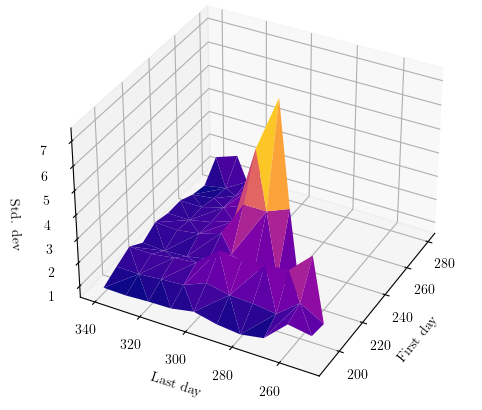
\includegraphics[width=0.5\linewidth]{pics/heatmap3d2}
\figcaption{3D -surface plot of day interval ranges and resulting standard deviations for FMI Kuopio dataset.}
\label{fig_heatmap3d2}
\end{figure}

\newpage

\subsection{Latitude estimation results}
The following two tables contain examples of the results of the latitude estimation algorithm. Results of the latitude estimation algorithm are not as good as the longitude estimations, but for now they will suffice. The predictions follow a similar patter as the previous longitude estimations in that predictions for the Helsinki installation are grouped tighter and their errors are lower than those of the Kuopio installation. 

\begin{table}[!ht]
\centering
\begin{tabular}{r|c|c|c|c} \hline\hline

\multicolumn{5}{ c }{FMI Helsinki latitude estimation results}\\\hline
Year & First min. p. & Error &  Last min. p. & Error \\

2021 & $59.792^\circ$ &  $-0.677^\circ$ & $60.186^\circ$ & $-0.334^\circ$\\
2020 & $59.792^\circ$ &  $-0.412^\circ$ & $60.186^\circ$ & $-0.018^\circ$\\
2019 & $59.896^\circ$ & $-0.308^\circ$ & $59.558^\circ$ & $-0.646^\circ$\\
2018 & $59.945^\circ$ & $-0.259^\circ$ & $59.463^\circ$ & $-0.741^\circ$\\
2017 & $60.577^\circ$ & $0.373^\circ$  & $60.008^\circ$ & $-0.196^\circ$\\

\hline\hline
\end{tabular}
\tabcaption{Estimated latitudes for FMI Helsinki Kumpula dataset with day range of 190th to 250th}
\label{table_geolocator_latitude_results_f_and_l2}
\end{table}

\begin{table}[!ht]
\centering
\begin{tabular}{r|c|c|c|c} \hline\hline

\multicolumn{5}{ c }{FMI Kuopio latitude estimation results}\\\hline
Year & First min. p. & Error &  Last min. p. & Error \\
2021 & $62.626^\circ$ &  $-0.266^\circ$ & $63.197^\circ$ & $0.305^\circ$\\
2020 & $62.259^\circ$ &  $-0.633^\circ$ & $61.895^\circ$ & $-0.997^\circ$\\
2019 & $62.983^\circ$ & $0.091^\circ$ & $62.708^\circ$ & $-0.184^\circ$\\
2018 & $62.722^\circ$ & $-0.170^\circ$ & $62.874^\circ$ & $-0.018^\circ$\\
2017 & $61.669^\circ$ & $-1.223^\circ$  & $61.152^\circ$ & $-1.740^\circ$\\

\hline\hline
\end{tabular}
\tabcaption{Estimated latitudes for FMI Kuopio Kumpula dataset with day range of 190th to 280th.}
\label{table_geolocator_latitude_results_kuopio}
\end{table}

\subsection{Possible issues and further development ideas}
PVlib POA based first and last minute estimations are slower to compute than necessary as only two timestamps are needed. The use of a simpler sunrise and sunset equation would increase the speed significantly, allowing for the use of brute force day range selection algorithms.

Different methods could also be used. In Hagdadi 2017 \cite{navid_australian_article} latitude estimations are done by fitting solar irradiance models with 3 unknown parameters to power generation measurement data. The latitude deltas of 1.65 to 3.42 degrees in the 2017 article are higher than those achieved in this thesis, however as the datasets, geographical regions and algorithms are different, direct comparison can not be made.

%by this paper, however as the datasets, geographical regions and algorithms are different, direct comparison can not be made.

In earlier Figure \ref{fig_slope_to_latitude} the slope to latitude fitting can be seen to be slightly off. This is because the polynomial used is of 2nd degree and higher degree polynomials may result in a closer fit. Similarly a piecewise linear interpolation based fitting could result in a more accurate model and thus better estimation accuracy at the risk of overfitting. 


\newpage
\section{Combined latitude and longitude estimations}
As it is unlikely that the longitude and latitude estimation algorithms are used in isolation from one another, their results should be examined together. This can be done by plotting the estimated locations on a map. Here the two installations in Helsinki and Kuopio and their predicted locations per year are plotted side by side with day range of 190 to 280.

\begin{figure}[h]
	
     \centering
     \begin{subfigure}[b]{0.45\textwidth}
         \centering
         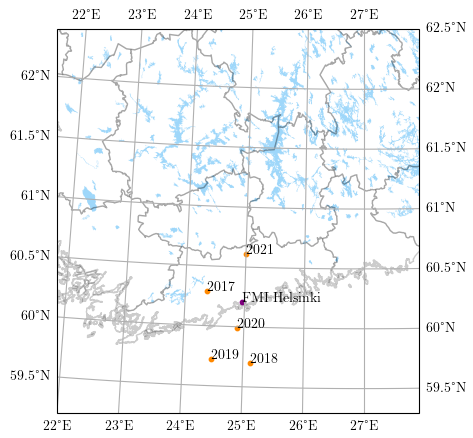
\includegraphics[width=\textwidth]{pics/geolocationmap2}
         \caption{FMI Helsinki.}
         \label{fig_geolocationhelsinki}
     \end{subfigure}
     \hfill
     \begin{subfigure}[b]{0.45\textwidth}
         \centering
         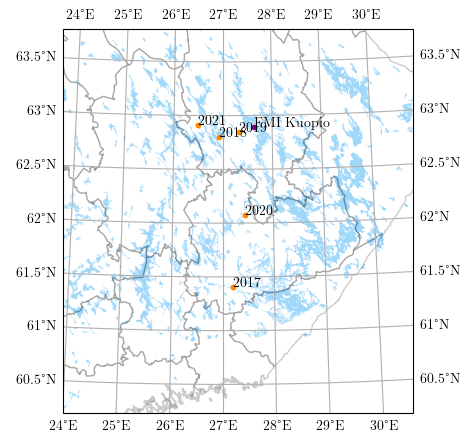
\includegraphics[width=\textwidth]{pics/geolocationmap3}
         \caption{FMI Kuopio.}
         
         \label{fig_geolocationkuopio}
     \end{subfigure}
     \hfill
     \caption{Geolocation estimations for FMI datasets.}
     \label{fig_anglespace}
\end{figure}

\noindent In the Helsinki predictions figure, the estimated geolocations are scattered around the known installation location, showing very little bias and some random noise. Similar behavior can be seen in Kuopio predictions where two outliers 2017 and 2020 deviate more significatly. One degree on the latidue axis is approximately 110 km regardless of latitude and longitude, one degree of longitude is 56km at $60^\circ$ N and 50 km at $63^\circ$ N. As the variance is strongest on the latitude axis, it is likely that the latitude prediction algorithm is more sensitive to variations in the data and further development should be focused on more accurate latitude prediction and day range selection.


The results can be compared to the data resolution. One minute delta in measurements corresponds to a longtudinal shift of 14 kilometers in longitudinal axis at $60^\circ$. As the point cloud width is approximately $1^\circ$ or 50km, the estimates can be thought to have a longitudinal range of 50km, $1^\circ$ or 3.5 minutes with nearly the same values for the Kuopio installation. As the temporal resolution of measurements is 1 minute, the algorithm should not be limited by temporal resolution.